% Copyright 2004 by Till Tantau <tantau@users.sourceforge.net>.
%
% In principle, this file can be redistributed and/or modified under
% the terms of the GNU Public License, version 2.
%
% However, this file is supposed to be a template to be modified
% for your own needs. For this reason, if you use this file as a
% template and not specifically distribute it as part of a another
% package/program, I grant the extra permission to freely copy and
% modify this file as you see fit and even to delete this copyright
% notice. 

\documentclass{beamer}
\usepackage{amsmath}
\usepackage{bm}
\usefonttheme{professionalfonts}
\usepackage{newtxtext,newtxmath}
\usepackage{ragged2e}
\newcommand{\bh}{\bm{h}}
\newcommand{\bt}{\pmb{\theta}}
\newcommand{\bG}{\pmb{\Gamma}}
\newcommand{\p}{\pause}
\newcommand{\pitem}{\pause \item}
\newcommand{\N}{\mathcal{N}}
\newcommand{\Y}{\bm{\mathcal{Y}}}
% There are many different themes available for Beamer. A comprehensive
% list with examples is given here:
% http://deic.uab.es/~iblanes/beamer_gallery/index_by_theme.html
% You can uncomment the themes below if you would like to use a different
% one:
%\usetheme{lankton-keynote}
%\usetheme{AnnArbor}
%\usetheme{Antibes}
%\usetheme{Bergen}
%\usetheme{Berkeley}
%\usetheme{Berlin}
%\usetheme{Boadilla}
%\usetheme{boxes}
%\usetheme{CambridgeUS}
%\usetheme{Copenhagen}
%\usetheme{Darmstadt}
%\usetheme{default}
%\usetheme{Frankfurt}
%\usetheme{Goettingen}
%\usetheme{Hannover}
%\usetheme{Ilmenau}
%\usetheme{JuanLesPins}
%\usetheme{Luebeck}
\usetheme{Madrid}
\usepackage[final]{pdfpages}
%\usetheme{Malmoe}
%\usetheme{Marburg}
%\usetheme{Montpellier}
%\usetheme{PaloAlto}
%\usetheme{Pittsburgh}
%\usetheme{Rochester}
%\usetheme{Singapore}
%\usetheme{Szeged}
%\usetheme{Warsaw}
%\usecolortheme{beetle}

\newcommand*\samethanks[1][\value{footnote}]{\footnotemark[#1]}

\setbeamertemplate{navigation symbols}{}%remove navigation symbols
\title[The Network of FDI Flows]{The Network of Foreign Direct Investment Flows:\\Theory and Empirical Analysis\thanks{\scriptsize {Acknowledgement: This material is based on work supported by the National Science Foundation under IGERT Grant DGE-1144860, Big Data Social Science.}}}


\author[Schoeneman, Zhu, \& Desmarais]{%
  \texorpdfstring{%
    \begin{columns}
      \column{.3\linewidth}
      \centering
      John Schoeneman{\thanks{\scriptsize{Pennsylvania State University}}} \\ \scriptsize{jbs5686@psu.edu\\ PhD Candidate}
      \column{.3\linewidth}
      \centering
      Boliang Zhu{\samethanks[2]} \\ \scriptsize{bxz14@psu.edu\\ Assistant Professor}
    \end{columns}
    \vspace{12pt}
    \begin{columns}
      \column{.3\linewidth}
      \centering
      Bruce Desmarais{\samethanks[2]}\\ \scriptsize{bdesmarais@psu.edu\\ Associate Professor}
    \end{columns}
 }
 {Author 1, Author 2, Author 3}
}

\date{April 8, 2017}



% - Use the \inst command only if there are several affiliations.
% - Keep it simple, no one is interested in your street address.

% - Either use conference name or its abbreviation.
% - Not really informative to the audience, more for people (including
%   yourself) who are reading the slides online


% This is only inserted into the PDF information catalog. Can be left
% out. 

% If you have a file called "university-logo-filename.xxx", where xxx
% is a graphic format that can be processed by latex or pdflatex,
% resp., then you can add a logo as follows:

% \pgfdeclareimage[height=0.5cm]{university-logo}{university-logo-filename}
% \logo{\pgfuseimage{university-logo}}



\begin{document}

\begin{frame}
  \titlepage

%Slide 1
%?Good afternoon and thank you for the opportunity to present this paper today on Foreign Direct Investment, (FDI) networks. My name is John Schoeneman and I am currently a PhD candidate at Penn State. My coauthors for this article are Dr. Zhu and Dr. Desmarais.?

\end{frame}




\begin{frame}{Introduction}


\begin{itemize}
 \item{Motivation}
 \begin{itemize}
 \item{Explain FDI networks}
\item{Violation of Independence Assumptions}
\item{Theoretical Importance of Dependence Terms}
 \end{itemize}
\item{FDI as a Network}
\begin{itemize}
\item{Reciprocity}
\item{Transitivity}
 \end{itemize}

  \item{Simultaneously test exogenous variables}
 \end{itemize}

%Slide 2
% "Foreign Direct Investment has grown over the years in magnitude and the number of destinations as well as senders, creating an intricate web of relationships for both trade and investment. Alongside of this increase, scholars have sought to explain who sends FDI and who receives it with a number of economic and political variables.  Historically, statistical models that have been used to test theories rely on the assumption that countries and pairs of countries are independent of one another. We argue that for most  foreign direct investment flows, and most applications, that this assumption is overly optimistic. This lack of independence though is not our only motivator to study the network of FDI. We argue that dependence terms such as reciprocity and clustering are theoretically important as well and present hypotheses for them. Furthermore, we test these network terms simultaneously with a selection of exogenous variables that have been found to be important in the literature." 


\end{frame}

\begin{frame}{Literature}

\begin{columns}[T]
    \begin{column}{.5\textwidth}
\begin{itemize}
\item{Dyad-level Covariates}
\begin{itemize}
\footnotesize{
\item{Gravity +} 
\item{Contiguity +} 
\item{Common Language +} 
\item{Four Types of Defense Treaties +}  
\item{Colonial Relationships +}
 \item{PTA depth +}
 }
\end{itemize}
\end{itemize}
    \end{column}
    \begin{column}{.5\textwidth}
\begin{itemize}
\item{Country-level Covariates (s/r)}
\begin{itemize}
\footnotesize{
\item{GDP per capita +/-} 
\item{GDP Growth Rate +/+} 
\item {Polity IV +/+} 
\item{Political Violence -/-} 
\item{Trade Openness +/+}
 }
\end{itemize}
\end{itemize}
        \end{column}
  \end{columns}
 
%Slide 3

%  "The list below is a selection of the exogenous covariates that have been examined in the literature. Standard economic models attribute cross-border capital movements primarily to relative factor endowments, market size, and transportation and trade cost. As with trade, much of this is controlled for using the gravity model, and a selection of other factors such trade openness. However, noting the risk of expropriation, the recent political economy of FDI literature emphasizes the importance of political institutions in constraining host government's opportunistic behavior. Scholars suggest that political constraints  and rule of law that are often found in democratic governance. Also analyzed in the literature is the participation in international institutions such as defense treaties and preferential trade agreements (or PTAs) that help to ensure policy credibility and provide investor protection, thereby luring in foreign investors. We add to political economy model two dependency terms."


\end{frame}

\begin{frame}{Reciprocity}

\begin{itemize}
\item{Reciprocity}\\

\centering{
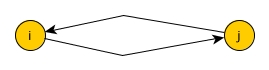
\includegraphics[scale=.7, clip=true, trim=0cm 0cm 0cm 0cm]{slides_figures/reciprocity.jpg}
}\\

\justifying
\item{Standard practice to resolve political opposition from competing firms}\\
\item{Example: Chinese firms' mergers (Tingley et. al. 2015)}
\end{itemize}


  %Slide 4
% "The first structural dependency we focus on is reciprocity, also known as mutuality. For the FDI network, this statistic is higher when the more FDI country i sends to country j, the more likely country j is to send more FDI to country i. As with trade, expansion of foreign firms into a country's market is generally met with some opposition by the owners of similar firms that do not want competition or other actors that are concerned about compromising national security. The political route to resolve this conflict is through reciprocal agreements. This allows politicians to build up sufficient support to remove barriers for FDI by granting the opposing firms or other sectors of the economy access to new markets. It also signals a 'tit for tat' scenario to prevent countries from blocking future investment. This was evident in findings that showed US officials were more likely to block acquisition of US companies by Chinese firms when Chinese had recently blocked investment for US firms."

\end{frame}

\begin{frame}{Transitivity}

\begin{itemize}
\item{Transitivity}

\centering{
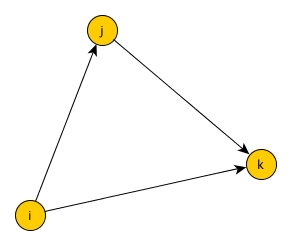
\includegraphics[scale=.5, clip=true, trim=0cm 0cm 0cm 0cm]{slides_figures/transitivity.jpg}
}\\
\justifying
\item{MNC expansion and supply-chain fragmentation}
\item{PTA networks}
\item{Example: Volkswagen and EU}

\end{itemize}
  %Slide 5
% "The second network dependency we estimate is transitivity, also known as the clustering coefficient. The transitivity network statistic is a triadic closure that is not a loop. Put another way, the stronger the two-path between country i and j, the higher the likelihood is of a stronger tie between i and j. 

%Large MNCs are the dominant players in global trade networks, often investing in multiple countries, even for only one type of finished product, and are increasingly involved in all levels of production as they seek to increase profits. This expansion increases the chance that an investor is more likely to invest in a country for which a two-path already exists since it is already part of the production network. For instance, Volkswagen's investment in Skoda Auto in Czech Republic not only attracted other auto makers such as PSA Peugeot and Toyota, but also international suppliers of parts and components to acquire local firms or build new factories; ``As of 2002, there were 270 firms operating in the Czech Republic, representing 45 percent of the top 100 world suppliers of automotive parts and components.''

 %Another key factor is that this vertical FDI is dependent on trade liberalization. Therefore PTAs can reinforce or expand these triadic clusters through the expansion of trade networks. The PTAs can reduce the risk of expropriation explicitly and by reinforcing a sustained interest in protecting investors. A prominent example is the creation of the European Union led to rapid increase of intra-region FDI." 

\end{frame}





\begin{frame}{The Count Exponential Random Graph Model (ERGM)}

The probability (likelihood function) of observing the network is:

$$ \text{Pr}_{\bm{\theta};h;\bm{g}}( \bm{Y}=\bm{y} )=\frac{ h(\bm{y})\text{exp}( \bm{\theta} \cdot \bm{g} (\bm{y}) )}{\bm{\kappa}_{h,\bm{g}}(\bm{\theta})} $$


Decomposition:
$$
\underbrace{\bm{h(y)}}_{Distribution} \qquad \underbrace{\bt}_{Effects} \qquad \underbrace{\bm{g(y)}}_{Net\hspace{3pt} Stats} \qquad \underbrace{\bm{\kappa}_{h,\bm{g}}(\bm{\theta})} _{Normalizer}
$$

Constants:
\begin{itemize}
\item{Sum, Sum$^{(1/2)}$, and Nonzero}
\end{itemize}
%Slide 6
% "We use the  count exponential random graph model (ERGM) for estimating the network dependencies and exogenous covariates. The Poisson reference function is used to parameterize the components of our model that are edge-specific, noted as h(y). Theta is the exogenous covariates and g(y) includes the network statistics. We include in the model terms that account for density of the network, variance, and zero-inflation."


\end{frame}

\begin{frame}{ERGM Dependence Terms}
$$ \text{Reciprocity}: \bm{g(y)} = \sum_{(i,j) {\in} \mathbb{Y}}min(\bm{y}_{i,j},\bm{y}_{j,i})$$

$$\text{Transitive Weights}: \bm{g(y)} =  \sum_{(i,j) {\in} \mathbb{Y}}\min\bigg( \bm{y}_{i,j}, \max\limits_{k{\in}N}\Big(\min(\bm{y}_{i,k},\bm{y}_{k,j})\Big) \bigg),$$ 
%Slide 7
% Reciprocity for the model is estimated for the minimum of the dyad, which is the conditional probability that a particular value of  Yij is deflated by theta for for every unit by which Yi,j is less than Yj,i. Or put differently, larger minimum values increase the value of reciprocation. 

% This specification for transitive weights measures the effect of the highest combined two-path between nodes which is defined as the highest minimum value of the two edges. Here the effect can be interpreted as the stronger the two-path, the higher the FDI from i to j and conversely the more FDI there is from i to j, the stronger the two-path (Krivitsky 2011)

\end{frame}




\begin{frame}{Model Fit and Bias}


    \centering
    BIC Difference between Models\\
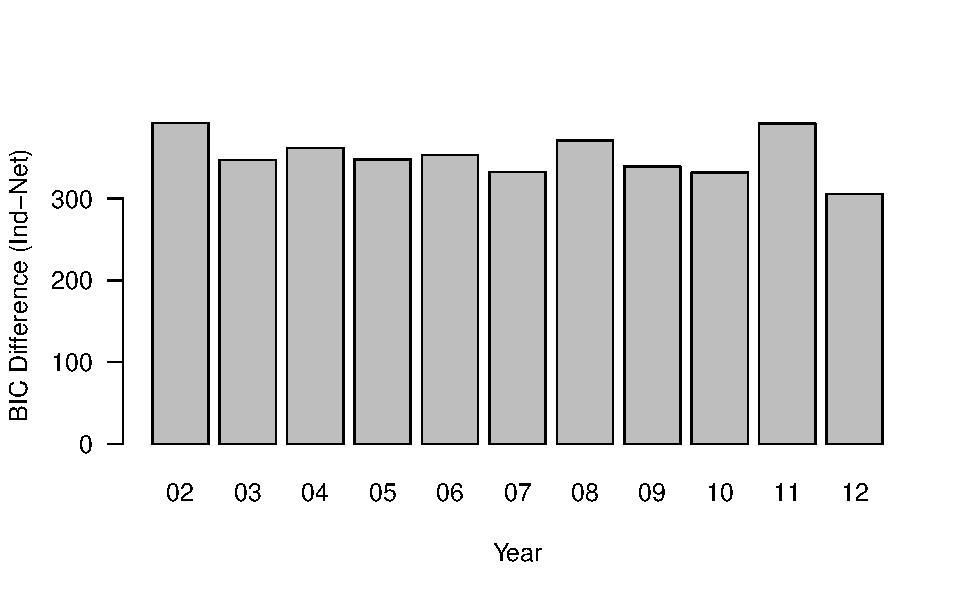
\includegraphics[scale=.6]{slides_figures/BICdiff.pdf}  

%Slide 8
% To evaluate model fit, we fit the model with network terms and with network terms. We then subtract the network model Bayesian Information criterion from that of the independent model, meaning that higher numbers indicate better fit. We use BIC since it is robust against increases in model fit simply due to added complexity. Here we see that for every year, inclusion of the network structural dependencies improves model fit.


\end{frame}



\begin{frame}{Count Model and Network Dependencies}

\centering
\begin{tabular}{c@{\hskip -.4cm}c}
\small{Reciprocity} & \small{Transitivity} \\ 
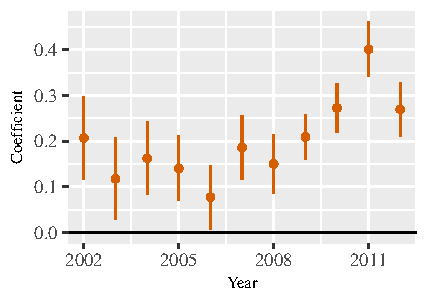
\includegraphics[height=.4\textheight, clip=true, trim=0cm .5cm .1cm .1cm]{slides_figures/rl_plots/Mutuality.pdf}   &
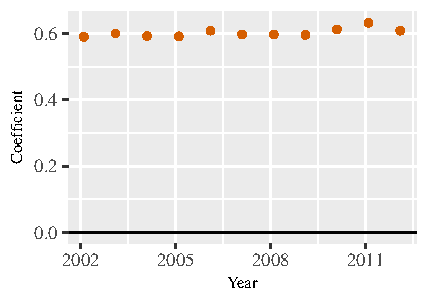
\includegraphics[height=.4\textheight, clip=true, trim=.5cm .5cm .6cm .1cm]{slides_figures/rl_plots/Transitivity.pdf} \\  
\end{tabular}

%Slide 9
% Also, and most important, is that the network terms,  reciprocity and transitivity, are significant and positive , with the bars representing 95% CI, for all years. This supports our hypotheses regarding the network dependencies and demonstrates that models that do not control for these dependencies violate independence assumptions.


\end{frame}


\begin{frame}{Network Statistics}
\centering
  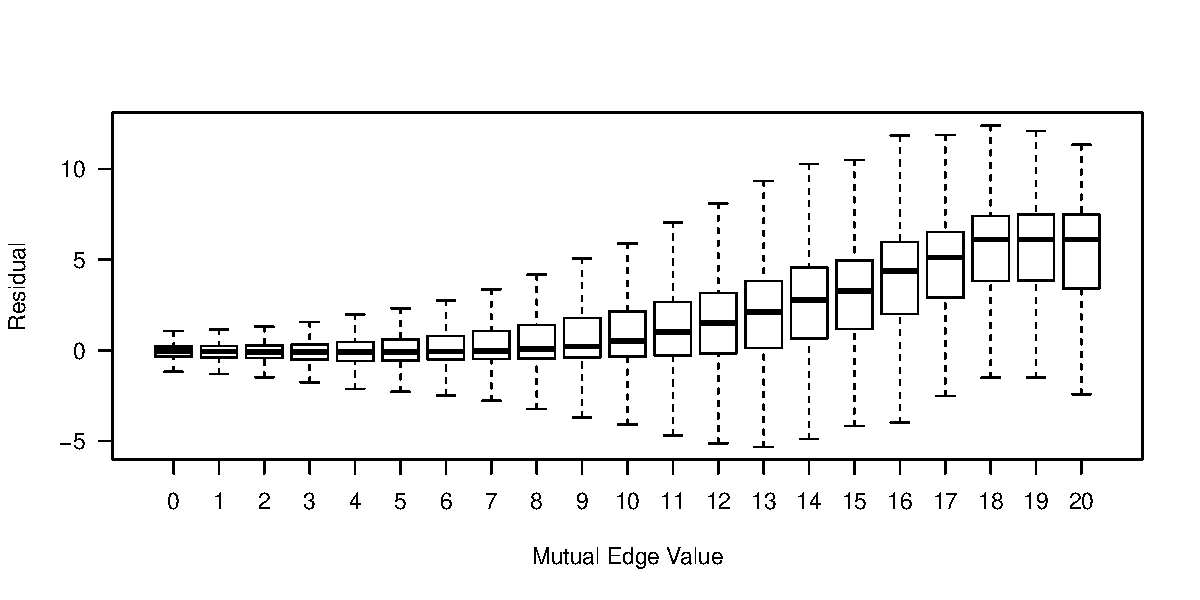
\includegraphics[scale=.45, clip=true, trim=0cm .5cm 0cm 1.9cm]{slides_figures/mutualBoxplot.pdf}\vfill
   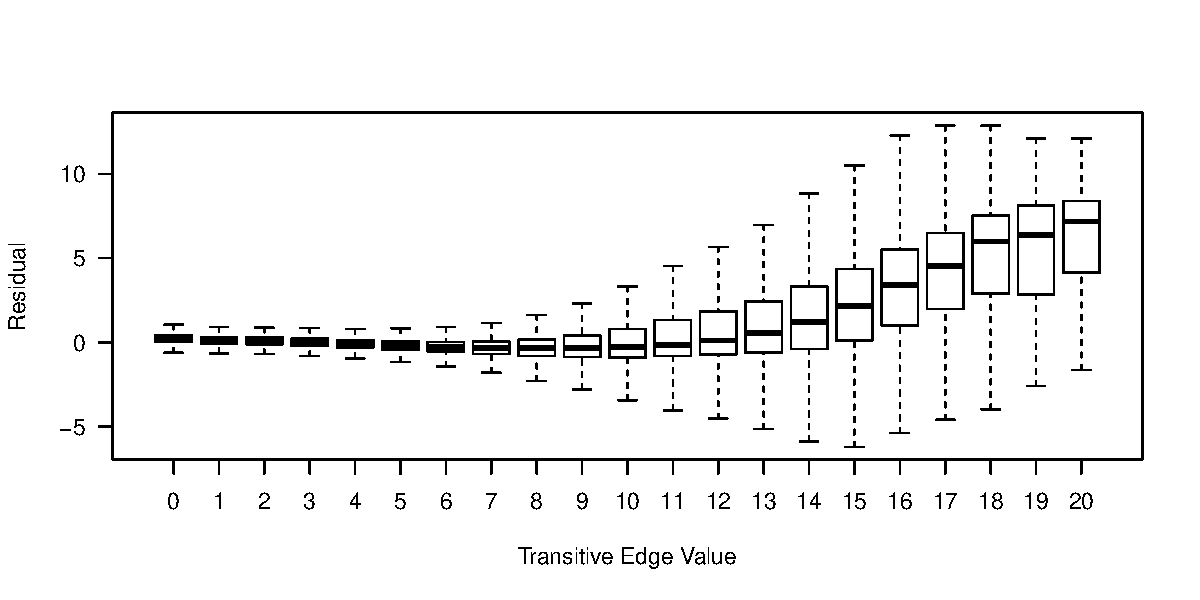
\includegraphics[scale=.45, clip=true, trim=0cm .5cm 0cm 1.9cm]{slides_figures/transitiveBoxplot.pdf}
%Slide 10
% Network statistics are not readily interpreted as OLS coefficients and so plots below provide a way to interpret them. The 'residual' here on the y-axis is the difference between the simulated edge values from the 2012 count ERGM and the value that would be predicted using only the exogenous covariates.The x-axis is fixed value of FDI from country j to i. And so if country j sent 15 units to country i, the model only using exogenous covariates would underestimate the simulated value between i to j by 3 units, all of this on the log scale. The same is true for transitivity, but here the predictive edge on the x-axis is the highest minimum value of the edge in the two-path from i to j.

\end{frame}


\begin{frame}{Covariate Results}

\centering
\begin{tabular}{c@{\hskip -.4cm}c@{\hskip -.4cm}c}
\small{Log-GDP Product} & \small{Distance} & \small{Contiguity} \\
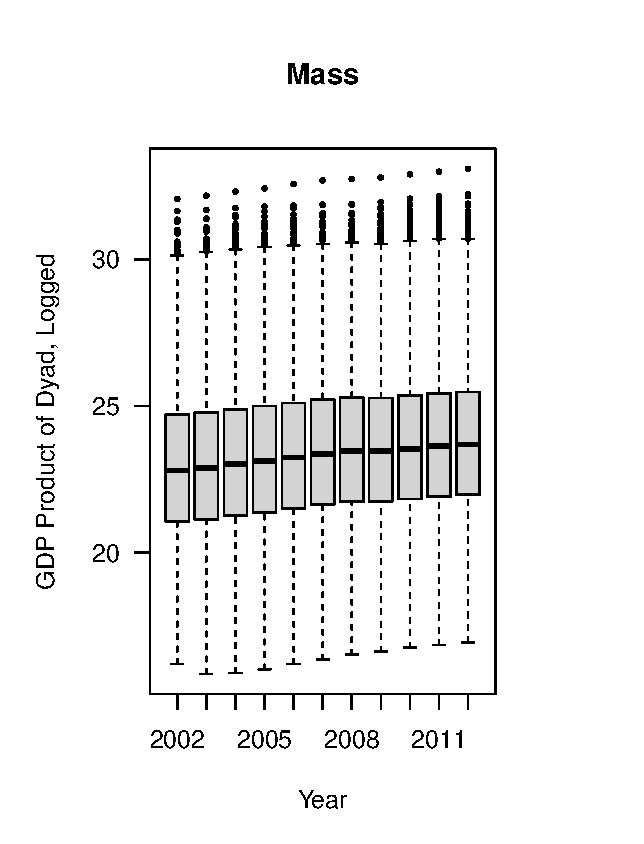
\includegraphics[height=.3\textheight, clip=true, trim=.5cm .5cm 0cm .1cm]{slides_figures/rl_plots/mass.pdf}    &
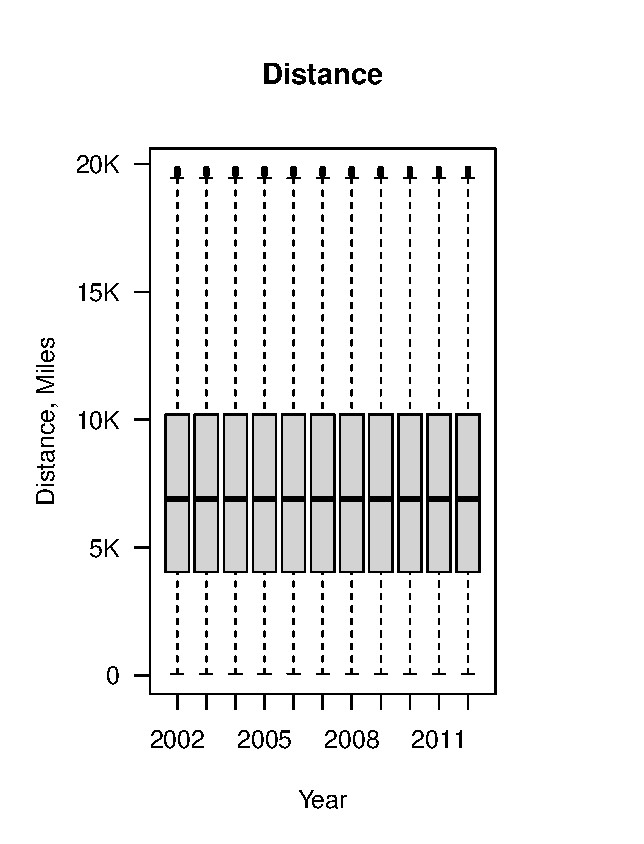
\includegraphics[height=.3\textheight, clip=true, trim=.5cm .5cm 0cm .1cm]{slides_figures/rl_plots/distance.pdf}   &
\includegraphics[height=.3\textheight, clip=true, trim=.5cm .5cm 0cm .1cm]{slides_figures/rl_plots/contiguity.pdf}\\


\small{Dest. Polity} & \small{Dest. Trade Openness} & \small{PTA Depth} \\ 
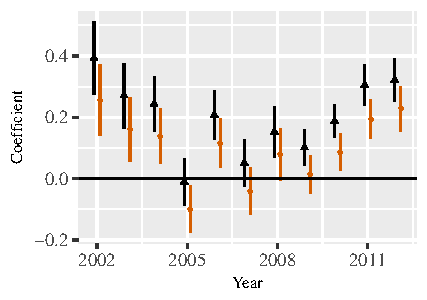
\includegraphics[height=.3\textheight, clip=true, trim=.5cm .5cm 0cm .1cm]{slides_figures/rl_plots/DestPolity.pdf} 
 &
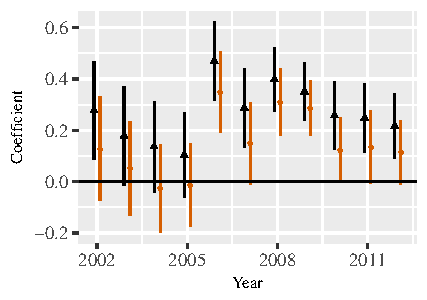
\includegraphics[height=.3\textheight, clip=true, trim=.5cm .5cm 0cm .1cm]{slides_figures/rl_plots/DestTO.pdf}   &
\includegraphics[height=.3\textheight, clip=true, trim=.5cm .5cm 0cm .1cm]{slides_figures/rl_plots/PTAdepth.pdf} \\  
\end{tabular}

%Slide 11
% To illustrate how estimates can be biased, I have included here six of the exogenous covariates from the models, although there were shifts in more than these six. The black points are for models without network dependency controls and the orange points are for the models that include them. One covariate here that has received a lot of attention in the literature here is the Polity. We see that the estimates shift in magnitude in the opposite direction and in some instances move from being significant at the 95% level to insignificant.  Therefore, by assuming away these dependencies, scholars are in danger of committing Type I errors despite readily available techniques to avoid this pitfall. 

\end{frame}






\begin{frame}{Conclusion and Future Research}

\begin{itemize}
\item{Network terms are substantively important}
\item{Network terms need to be modeled instead of being assumed away}
\item{Network dynamics and methodological constraints}
\end{itemize}


%Slide 12
% To conclude, FDI flows are part of a complex network. We offer both theoretical contributions to understanding the structural dependencies of the network that are substantively important and provide evidence that these dependencies cannot be assumed to be absent even if the scholar is uninterested in explaining them.

% For future iterations of the model we plan to adopt variations of the ERGM count model that allow us to account for network dynamics beyond the simple inclusion of the lagged FDI stock level. We are also exploring methodological paths that would allow us to condition the structural dependencies such as reciprocity on the development level mix within a dyad. Currently though the model and associated package do not allow for that in the binary models do. Thank you again for allowing me to present here today and I look forward to hearing your suggestions.


\end{frame}



\begin{frame}{Additional Covariates}

\centering
\begin{tabular}{c@{\hskip -.4cm}c@{\hskip -.4cm}c}
\small{Sum} & \small{Sum$^{(1/2)}$} & \small{Non-zero} \\
\includegraphics[height=.3\textheight, clip=true, trim=.5cm .5cm 0cm .1cm]{slides_figures/rl_plots/sum.pdf}    &
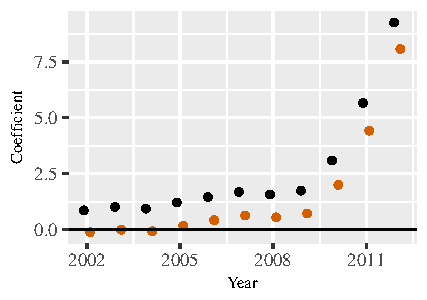
\includegraphics[height=.3\textheight, clip=true, trim=.5cm .5cm 0cm .1cm]{slides_figures/rl_plots/Sum_5.pdf}   &
\includegraphics[height=.3\textheight, clip=true, trim=.5cm .5cm 0cm .1cm]{slides_figures/rl_plots/nonzero.pdf}\\


\small{LDV} & \small{Dest. Political Violence} & \small{Origin Political Violence} \\ 
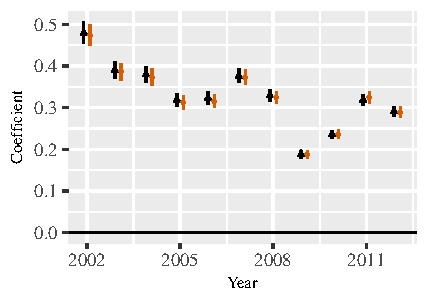
\includegraphics[height=.3\textheight, clip=true, trim=.5cm .5cm 0cm .1cm]{slides_figures/rl_plots/LDV.pdf} 
 &
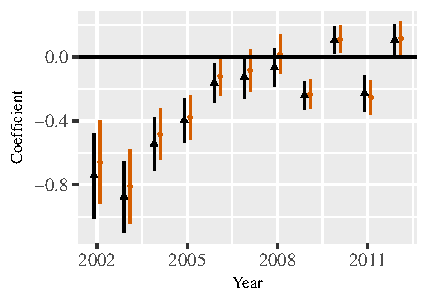
\includegraphics[height=.3\textheight, clip=true, trim=.5cm .5cm 0cm .1cm]{slides_figures/rl_plots/DestPV.pdf}   &
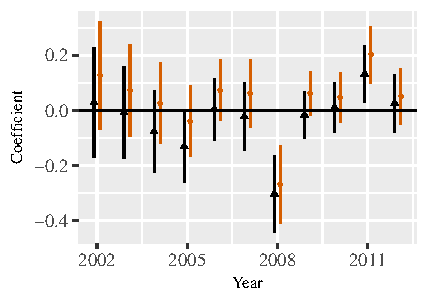
\includegraphics[height=.3\textheight, clip=true, trim=.5cm .5cm 0cm .1cm]{slides_figures/rl_plots/OriginPV.pdf} \\  
\end{tabular}

\end{frame}


\begin{frame}{ERGM Constants}

$$\text{Sum}:\bm{g(y)} = \sum_{(i,j) {\in} \mathbb{Y}}\bm{y}_{i,j}$$

$$\text{Sum, Fractional Moment}:\bm{g(y)} = \sum_{(i,j) {\in} \mathbb{Y}}\bm{y}_{i,j}^{1/2}$$

$$\text{Non-Zero}: \bm{g}_k = \sum_{(i,j) {\in} \mathbb{Y}} \mathbb{I}(\bm{y}_{i,j} \neq 0)$$

\end{frame}


\begin{frame}{ERGM Covariates}

$$ \text{Dyadic Covariate}: \bm{g(y,x)} = \sum_{(i,j)} \bm{y}_{i,j}x_{i,j}$$ 

$$ \text{Sender Covariate}: \bm{g(y,x)} = \sum_{i}x_i \sum_{j} \bm{y}_{i,j}$$

$$ \text{Receiver Covariate}: \bm{g(y,x)} = \sum_{j}x_j \sum_{i} \bm{y}_{i,j}$$
 

\end{frame}

\end{document}




